\documentclass[]{usiinfprospectus}

\usepackage[utf8]{inputenc}
\usepackage[english]{babel}
\usepackage[T1]{fontenc}

\captionsetup{labelfont={bf}}

\author{Carlos Eduardo B. Bezerra}

\title{A fault tolerant multi-server system for MMOGs}
%\subtitle{A crash-stop model oriented approach}
\versiondate{\today}
  
\begin{committee}
%With more than 1 advisor an error is raised...: only 1 advisor is allowed!
\researchadvisor[Universit\`a della Svizzera Italiana, Switzerland]{Prof.}{Fernando}{Pedone}
\academicadvisor[Universit\`a della Svizzera Italiana, Switzerland]{Prof.}{Fernando}{Pedone}
\committeemember[Universit\`a della Svizzera Italiana, Switzerland]{Prof.}{Committee}{Member1}
\committeemember[Universit\`a della Svizzera Italiana, Switzerland]{Prof.}{Committee}{Member2}
%\committeemember[Universit\`a della Svizzera Italiana, Switzerland]{Prof.}{Committee}{Member3}
\coadvisor[Universidade Federal do Rio Grande do Sul, Brazil]{Prof.}{Cl\'audio}{Geyer}
%\coadvisor[Universit\`a della Svizzera Italiana, Switzerland]{Prof.}{Research}{Co-Advisor2}
%\coadvisor[Universit\`a della Svizzera Italiana, Switzerland]{Prof.}{Research}{Co-Advisor3}
\phddirector{Prof.}{Michele}{Lanza}
\end{committee}

\abstract {
MMOGs -- massively multiplayer online games -- have become, in the last decade, an important genre of online entertainment, having a significant market share. In these games, many thousands of participants play simultaneously with one another in the same match. However, this kind of application is traditionally supported by a powerful (and expensive) central infrastructure with considerable cpu power and very fast and low latency Internet connections. This work proposes the use of a geographically distributed server system, formed by nodes which help serving the game to the players. The most important features that must be provided are: consistency (since different players should have the sense of one single shared virtual environment), timeliness (as these games are usually real-time applications) and fault tolerance (as some of the participating nodes may crash and become unavailable).
}
 

\begin{document}
\maketitle

%%%%%%%%%%%%%%%%%%%%%%%%%
\section{Introduction} \label{sec:introduction}
%%%%%%%%%%%%%%%%%%%%%%%%%

MMOGs emerged in the last decade as a new trend because of the decrease of the domestic Internet connection cost and the increase of its average bandwidth. This kind of games have become very popular because they allow the online interaction of a massive number of players at the same time. In the most succesful cases, such as World of Warcraft \cite{worldofwarcraft}, Lineage II \cite{lineage2} and EVE Online \cite{eveonline}, for example, tens of thousands of players are supported simultaneously \cite{chen2006pch}. In these games, the players can interact with one another in a virtual environment.

Generally, each player controls an entity called \emph{avatar}, which is his representation in the virtual environment -- a character who executes the orders given by the player, therefore interfering in the outcome of the game. To provide a consistent view among the different participants, every action performed by each avatar is processed by a server, which calculates the game state resulting from such action. This new state is then broadcast to the players to whom it might be relevant -- again, the state itself does not need to be consistent, but only what the players see.

To cope with the receiving and processing of thousands of actions and the broadcast of their respective resulting states, the traditional approach is to use a large central server -- usually a cluster with a high-speed, low latency Internet connection -- which provides such cpu power and network capabilities \cite{feng2007wnn}. Decentralized alternatives could be used, so that such expensive infrastructure would not be necessary. For example, a fully decentralized system could be used, where each player is a peer responsible for calculating a portion of the game state and for synchronizing it with other peers \cite{rieche2007ppb, hampel2006ppa, elrhalibi2005abm, iimura2004zfg, knutsson2004pps}.

In such peer-to-peer approach, the players would need to agree upon the outcome of the actions, in order for their view to be consistent. To reduce the traffic between peers, the state updates could be sent only to whom they are relevant. To define what is relevant for each player, the virtual environment could be divided into regions \cite{schiele2007rpp}, so that a small peer group would be formed by players who were inside each of these regions. Players whose avatars were in a given region could form a smaller peer-to-peer group -- possibly reducing also the cost of each agreement -- and their own computers would decide the outcome of the players' actions in that area of the virtual environment. Unfortunately, however, the fully decentralized approach would imply a heavy communication cost on the players, specially when running some agreement protocol. This might not only degrade the quality of the game, but also increase the requirements imposed on the players' computational resources, therefore likely reducing their number.

We propose here, then, a system composed of geographically distributed nodes which may act as game servers -- these nodes could be provided, for example, by volunteers or by companies which might have some commercial interest with the game being hosted. Some works, such as \cite{assiotis2006dam,ng2002msa, chertov2006olb, lee2003sdl} also propose the use of a distributed server, but they consider that the nodes are connected through a high speed and low latency network (e.g. a cluster), what makes their solutions only partially applicable in a scenario with highly dynamic and volatile resources, such as wide-area networks formed with volunteer resources. Such networks have some inherent problems: nodes with low availability and dependability, low bandwidth and low processing power compared to current dedicated MMOG servers maintained by large game companies.

The rest of this document is organized as follows: Section \ref{sec:mmogserver} describes the basic features of an MMOG server; Section \ref{sec:distserver} introduces our proposed distributed server model and describes briefly some of its protocols; Section \ref{sec:futurework} presents the research directions to be followed next and Section \ref{sec:achievements} lists some of the accomplishments achieved by this research so far.

%%%%%%%%%%%%%%%%%%%%%%%%%
\section{MMOG server overview} \label{sec:mmogserver}
%%%%%%%%%%%%%%%%%%%%%%%%%

We consider here persistent state real-time games with virtual environments where each player controls an avatar -- a virtual object that represents him -- by issuing commands to it. Through the avatar, the player interacts with the virtual world and with objects present in it, such as avatars from other players. The basic operation of the game network support system must be as follows: when a player connects to the server, it must send the current state of the player's avatar and of the surroundings of its current location; after that, this player keeps receiving periodic state updates for the objects which are relevant to it (usually based on whether those objects may be seen by the player \cite{bezerra2008a3,ahmed2008dai,minson2005aim}). When a player issues a command to the avatar (e.g. move avatar from one place to another, pick up an object, attack another player's avatar etc.), it is sent as a message to the server, which processes it and decides its outcome, probably changing the state of the game, which is then broadcast to all involved players.

\subsection{Services to be provided} \label{sec:services}

In order to give to the players the sense of a persistent virtual world through which they can wander and interact with each other, the MMOG server must provide, at least, the following services:

\begin{itemize}
	\item \textbf{Simulation} of the game, that is, the processing of commands sent by players to their avatars, calculating the corresponding outcomes, which may result in changes to the game state;
	\item \textbf{Broadcasting} a portion of the current game state to the different players connected to it, so that their view is consistent with the changes that might have happened;
	\item \textbf{Storage} of the game state, which is the combination of the states of all objects in the virtual environment.
\end{itemize}

It is important to note that in real-time games (as opposed to turn-based games), due to the possibly fast-paced interaction of the players, it is critical to provide \textbf{timeliness} for the delivery of state update messages to them, so that they have the illusion of a shared environment. For the same reason, it is necessary to provide \textbf{consistency} for the game state between each pair of players interacting with one another, which means that the game state they perceive must be as similar as possible. Although it is very hard to guarantee that every player will share the exact same view, it is important for their commands to be processed as if there was a single, strongly consistent game state, which is the one stored at the server. 


%%%%%%%%%%%%%%%%%%%%%%%%%
\section{Distributed server system} \label{sec:distserver}

The main purpose of the system is to reduce or, ideally, eliminate the necessity of a central server for the game. The approach we propose to achieve this is based on principles similar to those of volunteer computing, where a potentially large set of contributors make their computers available to perform tasks requested by some remote entity. With such a system, although each of these nodes is probably much less powerful than a traditional MMOG server, when working together they can sum up the cpu power and the network bandwidth necessary to host one of these games.

However, several questions arise when dealing with a potentially large, geographically distributed server system composed of voluntary nodes. First, as the nodes are volunteer, there is no guarantee that they will be available whenever they are needed, neither there is any guarantee regarding the amount of resources that each of these nodes makes available for the system -- be it cpu power, network bandwidth or storage capability. Group communication may also be a problem, since primitives for that -- such as network level multicast -- are not widely available on the Internet.

Finally, considering the potentially large number of nodes in this system, it is very likely that some of them present failures, for what we are assuming the crash-stop failure model -- therefore, we assume the possibility of nodes crashing and network links becoming unavailable. The services provided by the system must continue even in the presence of such failures. Not only must the distribution itself be transparent to the players, but also the existence of failures and their countermeasures must not be noticeable by them.

In Section \ref{sec:statepart}, we describe how the game state will be distributed among the different server nodes and, in \mbox{Section \ref{sec:consprot}}, a preliminary consistency management protocol, based on state machine replication, is presented. We also introduce, in Section \ref{sec:optmcast}, our group communication protocol on top of which our consistency management is performed.

%%%%%%%%%%%%%%%%%%%%%%%%%
\subsection{State partitioning} \label{sec:statepart}

In order to split a game server into several smaller units executed by many volunteer nodes, it is used the idea of dividing the virtual environment in regions, each of which being managed by a different server. Different approaches can be found in the literature, such as using fixed size cells and grouping them to form the regions \cite{devleeschauwer2005dma}, or using binary space partition trees \cite{bezerra2009fgl}. To tolerate failures, each server has several replicas, forming a server group.

The state partitioning is performed based on which objects are located in each region. The state of an object is managed, then, by the server group assigned to the region where that object is located. This way, the locality of data is explored: objects close to each other are more likely to interact and, as they are located on the same server group, their interaction should be faster. Besides, by exploring the locality of the game data (state of the objects), the inter-group communication overhead is reduced.

By having multiple server replicas in each region, the cost of broadcasting state update messages to the players is also reduced. Since all the replicas in a group are supposed to have an identical state, each one of them may send state updates to a different subset of the players located in that region. As the number of players may be as large as many thousands, this would probably be the most costly operation for the system and distributing it would have a significant impact on the system scalability.

%%%%%%%%%%%%%%%%%%%%%%%%%
\subsection{Consistency protocol} \label{sec:consprot}

As mentioned before, the players interact by issuing commands and having them processed by servers, which calculate the resulting game state and send it to the players. Every command can alter the state of the game, possibly based on a previous state. We assume, however, that the commands lead to a deterministic resulting game state. In other words, if the game starts in the state $S$, there is only one possible state $S'$ to be reached after a sequence $C=\{c_{1}, c_{2}, ..., c_{n}\}$ of commands.

The game state could then be modeled as a state machine, which would be replicated across the different server nodes, as proposed in \cite{lamport1978ird,schneider1990ift,lampson1996hbh}, and where each command would be responsible for a state transition. One way of implementing the distributed server system would be by creating such state machine and forwarding all commands to every server node, in the same (total) order. As the state transitions are deterministic, every server would be able to calculate the correct game state independently\footnote{It might be the case that some servers could still be processing an older command, while others might have already processed newer inputs. Although this might lead to an old state, it would never lead to an incorrect state. To check which one is the newest, it would be enough to have a version number considering, for instance, the number of commands processed, since the commands arrive in the same order at the different servers.}. We would, then, have a fully replicated server system. 

The problem with a fully replicated state machine approach for a distributed game server is that it would hardly scale well. As the number of servers increased, so would the cost of processing a command, as it would have to be totally ordered among other commands received by any of the other servers. Not only the number of control messages would grow and potentially saturate the servers' network bandwidth, but also the time needed for the total order of the commands to be achieved would possibly increase beyond a tolerable value.

We decided, therefore, to use a partial state machine replication scheme, so that only the server group responsible for a given state will have to process the commands that alter such state. To make this possible, each command must specify a \emph{target set} -- defined either by the player or by a server --, which contains the objects whose states are needed or altered by the command. As every object is assigned to a different server group, the protocol will then be able to infer which servers must process each command.

Instead of forwarding each command to every server, now only the servers that manage some object in the target set of a command would process it. The problem with such partial state machine replication is that, in order to execute some command, a group might need the previous state of an object managed by some other group. To solve this, a possibilty would be to have the groups requesting the states they need from other groups. Another solution, probably more latency-efficient, would be every group proactively sending the new states of the objects managed by it to other groups which might need them.

Sending new states to other groups proactively based on the possibility that they might need such states, however, may lead to all groups sending to each other the state changes of every object, degenerating to a fully replicated approach. Nevertheless, we can explore the fact that, in games, objects interact only with other objects situated nearby: we can define the regions of the virtual environment in such a way that only objects either in the same or in neighboring regions would be able to interact -- two regions are neighbors if, and only if, they share a border. As commands are executed by avatars, which are simply objects controlled by players, the result will be that, for each pair of objects in the target set of any command, these two objects will be either located in the same or in neighbor regions. This way, only groups managing regions that share a border would need to forward commands to each other\footnote{Although unlikely, it is possible to have a command sequence $C = \{c_1,c_2,\ldots,c_n\}$ where (1) every $c_i$ depends on the state resulting from $c_{i-1}$, (2) not every $c_i$ is processed by the same group and (3) not all of these groups manage neighbor regions. Nevertheless, the servers can detect such dependencies and forward the object states to the servers which need them. In the worst case, every group but one -- there is no dependency cycle -- would be waiting for another group, so the time needed to process a command would be proportional to the number of groups.}.

% Figure \ref{fig:consistency} illustrates two avatars situated in regions managed by different server groups, but still close enough to interact. Each command issued by their players has to be forwarded to the groups that manage some object in its target set, which is done by multicast.
% 
% \begin{figure}[!h]
%   \centering
%   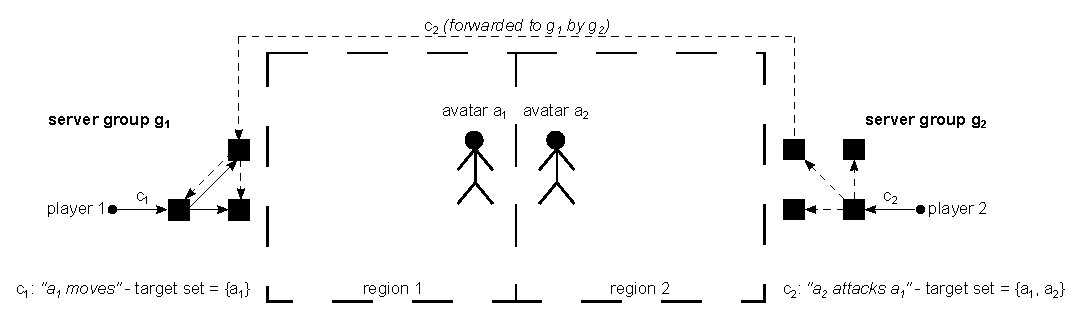
\includegraphics[width=0.8\linewidth]{images/consistency}
%   \caption{Multicasting a command to a group which manages an object in that command's target set}
%   \label{fig:consistency}
% \end{figure}

%Each command will be processed by the group which contains its targets, being ordered among other commands who also are relevant to that same group. When a command has targets from different groups, than it must be ordered in all of the groups involved, i.e. all the groups which manage one of that command's targets.

%As proposed in [cite related work], it is used here the idea of \textbf{contact servers} and \textbf{target servers}. In our architecture, the players whose avatars are in a certain region are distributed among the server nodes responsible for that region. The distribution is decided based on the network latency for each pair client-server. Each client is assigned to a server to which it has the lowest network latency among all servers in its region. This server, to which the client communicates directly, is its contact server. The target server is always the region manager, which can also be the contact server for certain players. When one of the servers gets overloaded because of the broadcasting of messages to players, these messages are then sent via other routes, even if the network latency of that new route is higher. Figure \ref{fig:arch} illustrates this architecture.
%
% \begin{figure}[!t]
% 	\centering
% 	\includegraphics[width=0.45\linewidth]{images/arch}
% 	\caption{Basic architecture with Region Managers and Region Replicas}
% 	\label{fig:arch}
% \end{figure}



%%%%%%%%%%%%%%%%%%%%%%%%%
\subsubsection{Quasi-genuine multicast} \label{sec:optmcast}

As the servers are organized in groups, and every command is sent to one or more of such groups, we can use a multicast protocol. Also, as commands seen by different servers must be handled in the same order, we need total order, so that the state machine replication approach can be used. Besides, the commands sent by each player should be executed in the same order in which this player issued them; therefore, the multicast protocol should provide FIFO ordering.

However, the inter-group communication overhead should be minimized, so that the distributed server would be more scalable. Non-genuine multicast primitives \cite{schiper2009gng} require that control messages keep being exchanged between groups, even when there is no application level message to be sent. On the other hand, although genuine multicast algorithms minimize the number of messages exchanged, they impose a greater latecy on their delivery \cite{schiper2008ica}.

We devised, then, a multicast protocol that, although not genuine, allows the system to increase its scale without getting flooded with control messages. We call it \emph{quasi-genuine}, because every group keeps sending messages to (and receiving from) other groups, even if there is no application level message to be exchanged, but only the ones with which it \emph{is possible to} exchange messages. The information concerning which other groups a given group can communicate with is given by the application.

The advantage of a quasi-genuine multicast protocol is that it would be a middle ground between genuine and non-genuine protocols, inheriting some advantages from both -- namely, improved scalability and lower message delivery time --, at the cost of restricting which groups can communicate with each other. Although the system can be reconfigured to change the group pairs that are able to exchange messages, such reconfiguration will have some cost, so this multicast protocol is more suitable for applications where this would not be frequent.

This can be used by our consistency management algorithm because every server group only has to forward commands to a specific set of other groups, which are the ones managing neighbor regions, and this is known as soon as the partitioning has been performed. Changes to the partioning should be performed rarely, as it would incur in some players migrating between servers. Therefore, the set of group pairs that can communicate with each other will not change frequently.

To further decrease the message delivery time, an optimistic delivery will also be employed. By assigning timestamps based on the local clocks -- which are supposed to be more or less synchronized -- and by every server waiting long enough for messages to arrive from another servers before performing the delivery, the final total message order will most likely match the timestamp order, so that the messages could be delivered in only one communication step, although that delivery would have to be confirmed by some conservative delivery.



%%%%%%%%%%%%%%%%%%%%%%%%%
% \subsection{Proposed causality definition and synchronization algorithm} \label{sec:algorithm}
% 
% When a player issues a command $c_{i}$, it is sent to its contact server, which forwards the command to the region manager. The region manager then processes the command sent by the player and calculates its resulting state, also considering every command -- or any kind of event -- $c_{j}$ sent by other players, such that $c_{j}$ was issued prior to $c_{i}$. Any prior event $c_{j}$ that the contact server should be aware of and that has not been received by the contact server of that player yet is then sent by the region manager. By having these prior events, the contact server is able to calculate the new game state that should be sent to the player who issued the command $c_{i}$.
% 
% The \textbf{causality} is defined here based on which objects are affected by an event. If commands $e_{i}$ and $e_{j}$ affect the same object, then they must be ordered. The order is defined by the time when they are delivered at the region manager responsible for that object.
% 
% asdf
% 
% We could also use the other idea (player --tob--> region servers; then region servers --lazy-synch-->all other servers)
% 
% 
% 
% %%%%%%%%%%%%%%%%%%%%%%%%%
% começar a falar das características específicas do sistema servidor distribuído, o que ele deve fazer (replicação, sincronização, tolerância a falhas, modelo crash-stop)
% 
% when adding a large number of players (falar aqui de timeliness), specially if they are distributed among different servers, many questions become critical. (falar aqui da sincronização com vários servidores)
% 
% - direct communication (players -> signed -> check by servers OU )
% 
% 
% As mentioned before, this work considers the crash-stop failure model. Therefore


%%%%%%%%%%%%%%%%%%%%%%%%%
\section{Published work} \label{sec:achievements}

Some related work that we have published so far include:
\begin{itemize}
  \item C. E. B. Bezerra, J. L. D. Comba, C. F. R. Geyer. A fine granularity load balancing technique for MMOG servers using a kd-tree to partition the space. \textit{VIII Brazilian Symposium on Computer Games and Digital Entertainment - Computing Track}, 2009.
  \item C. E. B. Bezerra, C. F. R. Geyer. A load balancing scheme for massively multiplayer online games. \textit{Multimedia Tools and Applications - Special Issue on Massively Multiplayer Online Gaming Systems and Applications}, v. 1, n. 1, pp. 263-289, 2009.
  \item C. E. B. Bezerra, F. R. Cecin, C. F. R. Geyer. A3: a novel interest management algorithm for distributed simulations of MMOGs. \textit{12-th IEEE International Symposium on Distributed Simulation and Real Time Applications}, 2008.
\end{itemize}
%%%%%%%%%%%%%%%%%%%%%%%%%

%%%%%%%%%%%%%%%%%%%%%%%%%
\section{Future work} \label{sec:futurework}

We are currently workings towards the validation of both the quasi-genuine multicast and the game state consistency management protocols, which require both formal proofs regarding correctness and experimental results to demonstrate their performance. Another direction that we intend to follow is to consider not only crash-stop faults, but also Byzantine faults. By tolerating these faults, the server system would also be resistant to cheating, which can also be seen as Byzantine behavior.

%%%%%%%%%%%%%%%%%%%%%%%%%

%%%%%
\bibliographystyle{abbrv}
\bibliography{references}



\end{document}
